\subsection{Photodiode} % (fold)
\label{sub:Photodiode}
\begin{frame}
    \frametitle{Photodiode}
    \framesubtitle{}
    \begin{columns}[c]
        \column{0.6\textwidth}
            \begin{block}{Aufgabenstellung}
                 \begin{itemize}
                    \item Untersuchung 
                    \begin{itemize}
                        \item der Lichtschranke
                        \item des Operationsverstärkers
                        \item der Störquellen
                    \end{itemize}
                 \end{itemize}
            \end{block}
        \column{0.4\textwidth}
            \begin{figure}[H]
            \begin{center}
                    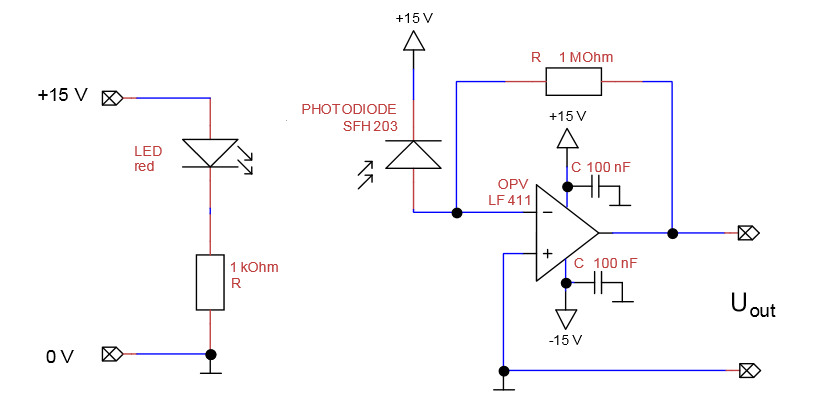
\includegraphics[scale=0.2]{./img/schaltung/photo.png}
            \end{center}
            \end{figure}
    \end{columns}
\end{frame}
\begin{frame}
    \frametitle{Messungen}
    \framesubtitle{}
    \begin{columns}[c]
        \column{0.6\textwidth}
            \begin{tabular}{c|c|c}
                & zur Wand & zur Fenster  \\
                \hline 
                offen& $-3.1V$ & $-3.6V$  \\
                abgedeckt & $-0.6V$ & $-0.3V$ 
            \end{tabular}
            \begin{block}{Störquellen}
                \begin{itemize}
                    \item Störung durch
                     \begin{itemize}
                        \item Sonnenlicht  
                        \item $100Hz$ Wechselspannung $\rightarrow$
                        Leuchstoffröhren
                        \item Schattenwurf durch Aufbau/Personen
                     \end{itemize}
                     \item Lichtmessung nur in abgedunkeltem Raum/Kasten
                     möglich oder
                     \item Filterung der Störsignale
                \end{itemize}
            \end{block}
        \column{0.4\textwidth}
            \begin{figure}[H]
            \begin{center}
                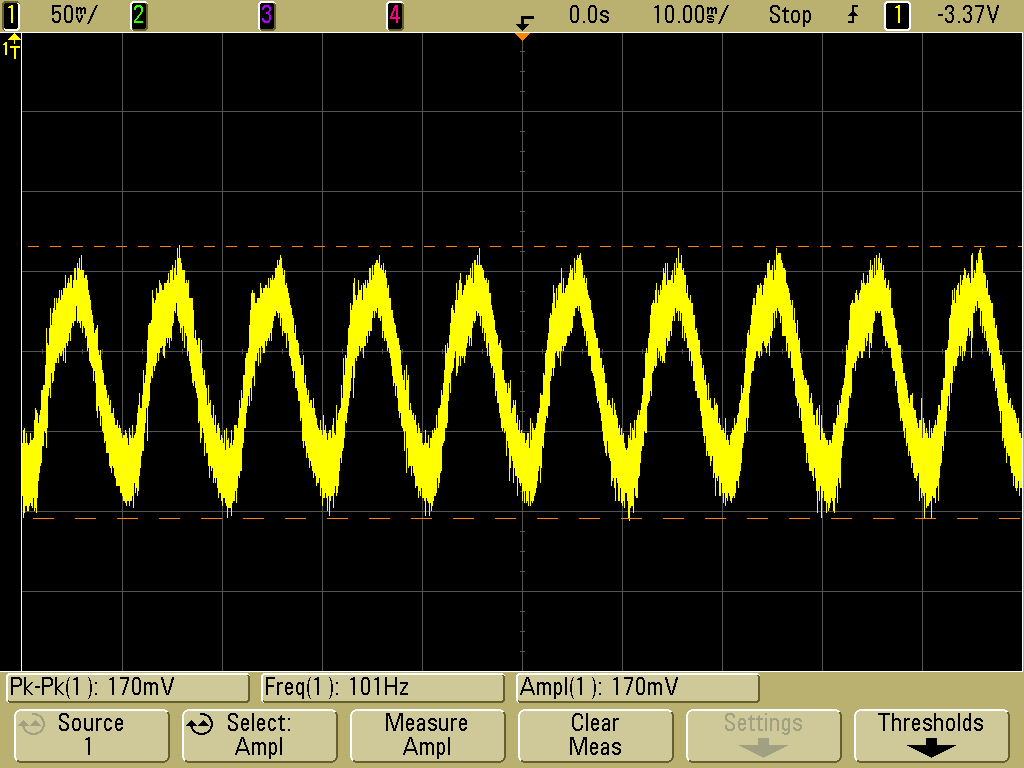
\includegraphics[scale=0.12]{./img/oszi/scope_0.png}
                \caption{Signal mit Diode zum Fenster ausgerichtet}
            \end{center}
            \end{figure}
     \end{columns}
\end{frame}
\begin{frame}
    \frametitle{Operationsverstärker}
    \framesubtitle{}
                 \begin{block}{}
                 \begin{gather*}
                     U_{out} = - \frac{R}{R_D} \cdot U_{in} 
                     \qquad
                     I_{in} = \frac{U_{in}}{R_D + R_2} \\
                     G = \frac{U_{out}}{U_{in}} = - R - \frac{R^2}{R_D}
                 \end{gather*}
                 mit
                 \begin{align*}
                     R &= 1M\Omega \\
                     R_D &= \text{Widerstand der Photodiode}
                 \end{align*}
            \end{block}
    \end{columns}
\end{frame}
% subsection Photodiode (end)
